

\section{Stress and equilibrium}

	\begin{frame}
		\begin{itemize}
		\item We are dealing with different configurations. One configuration is maybe unstressed and the deformed one is. So at the deformed x we should get an equilibrium of stresses and the external loads
		\item Now, the actual stresses at the deformed or current configuration is the Cauchy stress : defined as the force in different directions by the area in different planes
		\item Stresses can also be defined with respect to the initial configuration X			
					
		\end{itemize}

	\end{frame}

	\begin{frame}{Cauchy stress tensor}
		\begin{figure}
			\centering
			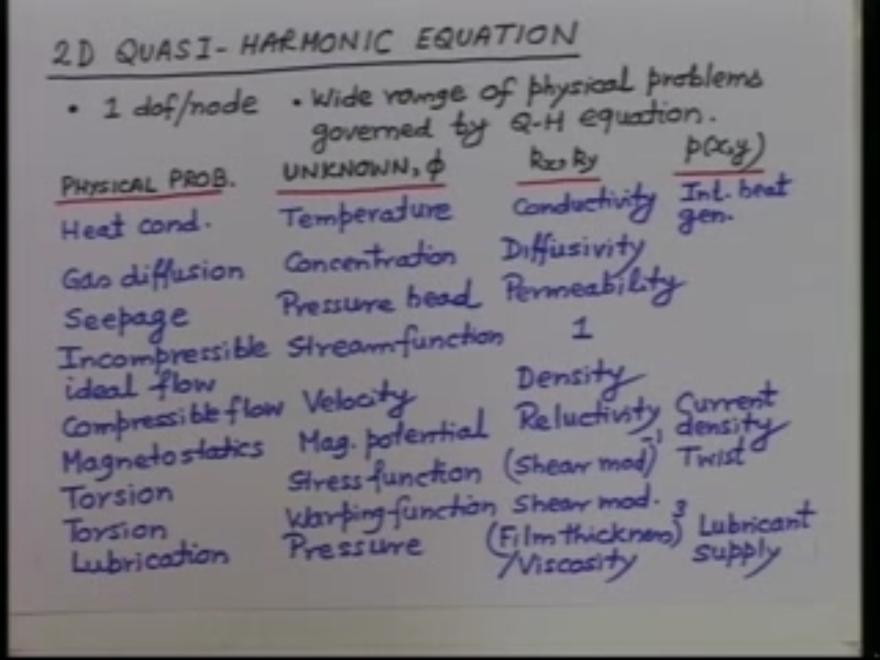
\includegraphics[width=0.5\linewidth]{\pth/continuum/fig7}
		\end{figure}
		At the deformed configuration :
		\begin{itemize}
			\item See two bodies $R_1$ and $R_2$ free body with force acting on them
			\item Imagine the traction vector on a small area element : ${t(n) = \frac{\Delta p}{\Delta a}}$ as lim $\Delta a \rightarrow 0$ where $\Delta p$ is the resultant force
			\item Obviously $t$ and $n$ will depend on the surface it acts on. Here on the right we can see that based on the surface we get opposite forces. (In the negative normal , we will get negative force which is positive in that direction!)

		\end{itemize}
	\end{frame}

	\begin{frame}
		\begin{figure}
			\centering
			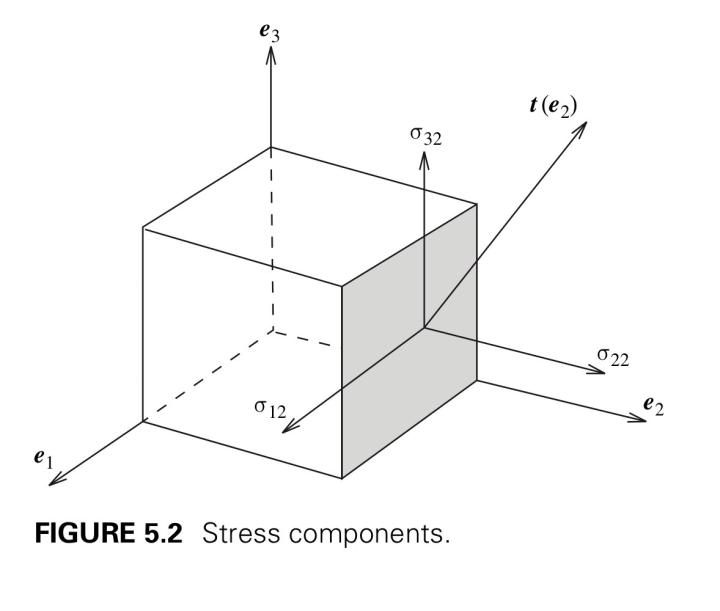
\includegraphics[width=0.5\linewidth]{\pth/continuum/fig8}
		\end{figure}
	
		\begin{itemize}
			\item Let us denote the traction acting on the surface having normals denoted by $e_1, e_2,e_3$
			\item Remember in the other slice we will have an opposite reaction
			\begin{equation}
			\begin{aligned}
			\ve{t(e_1) = \sigma_{j1}e_j} \\\ve{t(e_2) = \sigma_{j2}e_j}\\\ve{t(e_3) = \sigma_{j3}e_j}
			\end{aligned}
			\end{equation}
			\item Or $\ve{t_i = \sigma_{ji}e_j}$ or $\ve{t = \sigma^T e}$
		\end{itemize}
	\end{frame}

	\begin{frame}
		\begin{figure}
			\centering
			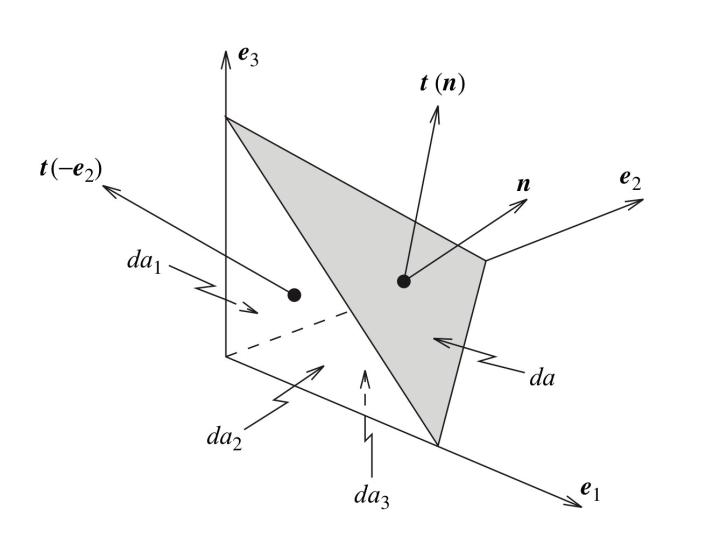
\includegraphics[width=0.5\linewidth]{\pth/continuum/fig9}
		\end{figure}
		
		Now let us look if we take a plane cut of that sphere. Again by context of opposite reactions. All the forces should be equal. So we will use here the concept of equilibrium between the traction vector we have defined in the last slide with respect to some basis and the traction vector defined on the angled plane.
		
		\begin{block}{Equilibrium}
			\begin{equation}
			\ve{t(n)}da + t(\ve{-e_i})da_i + \ve{f}dv = 0
			\end{equation}
			This states that the force vector on the inclined cut should be in equilibrium with the opposite forces defined on the negative sufraces and the body force
		\end{block}
	
	\end{frame}

	\begin{frame}
		\begin{itemize}
			\item  Now the areas (Because they are with defined respect to the basis vectors) can be written as the projection of the inclined area
			\begin{equation}
				da_i = da(\ve{n.e_i})
			\end{equation}
			\item Diving by da we get 
			\begin{equation}
			\ve{t(n)} + t(\ve{-e_i})\frac{da(\ve{n.e_i})}{da} + \ve{f}\frac{dv}{da} = 0
			\end{equation}
			\item $\frac{dv}{da} \rightarrow 0$  ( I don't know why????????????????)
			\item We get :
			\begin{equation}
			\begin{aligned}
			\ve{t(n)} = - t(\ve{-e_i})(\ve{n.e_i}) =  t(\ve{e_i})(\ve{n.e_i})\\
			\ve{t(n)} = (\ve{\sigma_{ji}e_j})(\ve{n.e_i}) \\
			\ve{t(n)} = (\ve{\sigma_{ij}e_i})(\ve{n.e_j}) \text{Replacing indexs}\\
			\end{aligned}
			\end{equation}
		\end{itemize}
	\end{frame}


	\begin{frame}
		\begin{itemize}
			\item Very interesting, we started off with a statement that the resultant force on the plane is equal to the summation of the opposite forces
			\item Then we got the traction vector is equal to the traction vectors multiplied by some scalar product (Think of ratio)
			\item $t(\ve{e_i})(\ve{n.e_i})$ states the traction in $e_i$ direction multiplied by the projection of planar area for i =1,2,3
			\item Now we can replace the traction vector by the components of stress vectors in the basis direction $\ve{t(n)} = (\ve{\sigma_{ij}e_i})(\ve{n.e_j})$
			\item Here we have to point out that $\sigma_{ij}$ has not been described as a tensor yet\\		
		\end{itemize}
	\end{frame}

	\begin{frame}{Tensor insight}
		\begin{itemize}
			\item If we look at $\ve{t(n)} = (\sigma_{ij}\ve{e_i})(\ve{n.e_j})$ , we can see that $\sigma_{ij}$ is just a component and $\ve{n.e_j}$ is a scalar (Or a projection).
			\item That scalar value then becomes the component of $e_i$. Lets see what that means 
			\begin{equation}
			\begin{aligned}
			\sigma_{12}\ve{e_1(n.e_2)}= \sigma_{12}\mat{1;0;0}(\mat{n_1,n_2,n_3}\mat{0;1;0}) = \sigma_{12} n_2 \mat{1;0;0}
			\end{aligned}
			\end{equation}
			\item So we took the second component of $n$ and added to the result of linear map in $e_1$.This is what we do when we multiply the first row of a matrix and a vector. We add all the components of the vector to keep in the first component of the output
			\item So we can write it therefore as
			\begin{equation}
				\ve{e_i(n.e_j) = (e_i \otimes e_j).n} 
			\end{equation}
			which states that the tensor takes the projection of $e_j$ in n and maps as components of $e_i$
			\item This then allows us to understand that $\sigma_{ij}(\ve{e_i \otimes e_j})$ is a tensor $\sigma$
		\end{itemize}
	\end{frame}

	\begin{frame}
		\begin{itemize}
			\item In simplicity $\ve{t(n)} = (\sigma_{ij}\ve{e_i})(\ve{n.e_j})$ says that for every cut, $\ve{n}$ 
			\begin{equation}
			\mat{t_1;t_2;t_3} = \mat{\sigma_{11}\ve{e_1(n.e_1)} + \sigma_{12}\ve{e_1(n.e_2)} + \sigma_{13}\ve{e_1(n.e_3)};\sigma_{21}\ve{e_2(n.e_1)} + \sigma_{22}\ve{e_2(n.e_2)} + \sigma_{23}\ve{e_2(n.e_3)} ; \sigma_{31}\ve{e_3(n.e_1)} + \sigma_{32}\ve{e_3(n.e_2)} + \sigma_{33}\ve{e_3(n.e_3)}}
			\end{equation}
			FIXXX. These are not components yet!
			\item And now you can see that $\ve{e_i \otimes e_j}$ just makes the tensor take the right projection and keeps in the component in the output
			\item $\sigma_{ij}n_j$ is therefore something like taking the projection of j for every component i
		\end{itemize}
	\end{frame}

	\begin{frame}{Problem \#1}
		\begin{figure}
			\centering
			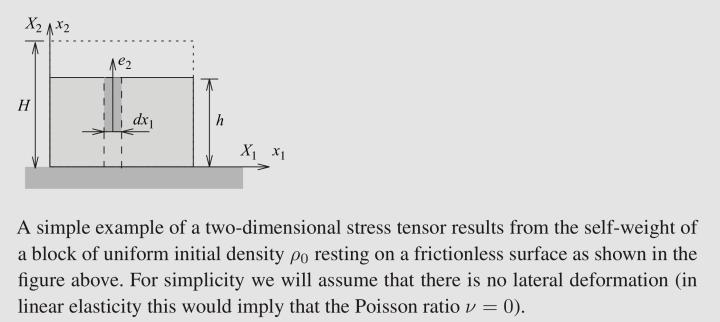
\includegraphics[width=0.7\linewidth]{\pth/continuum/fig10}
		\end{figure}
	\begin{itemize}
		\item $t(\ve{e_2}) = \dfrac{\left(-\int_{y}^{h} \rho g dx_2 \right)\ve{e_2}dx_1}{dx_1}$
		\item Mass conservation $\rho dx_1dx_2 = \rho_o dX_1dX_2$ + poisson = 0 give :
		\begin{equation}
		t(\ve{e_2}) = \rho_o g (H- X_2) \ve{e_2}
		\end{equation}
		\begin{equation}
		t(\ve{e_2}) = \sigma_{12}\ve{e_1} + \sigma_{22}\ve{e_2}
		\end{equation}
		so $\sigma_{12} = 0$ , so you can construct $\sigma$. Check Bonet Pge 138
	\end{itemize}
	\end{frame}

	\begin{frame}{Principal basis}
		\begin{itemize}
			\item Obviously the Cauchy stress components can be described with respect to its principal directions $\phi_1,\phi_2,\phi_3$ with principal stresses $\sigma_{\lambda_1},\sigma_{\lambda_2},\sigma_{\lambda_3}$
			\item So we can write in tensor notation :
			$\ve{\sigma = \sigma_{\lambda_i} \left(\lambda_i \otimes \lambda_i \right)}$
			(Only diagonals, the tensor is $i \otimes i$ which only is for the diagonal components)
			\item The cauchy stress is a spatial tensor (In the deformed configuration), and is symmetric because of the rotational equilibrium
		\end{itemize}
	\end{frame}

	\begin{frame}{Stress Objectivity}
		\begin{itemize}
			\item So the stress tensor should not change it's property when there is a rigid body motion etc.
			\item ???????????????? 
			
		\end{itemize}
	\end{frame}

	\section{Equilibrium}
	\begin{frame}{EQUILIBRIUM: Translational}
		\begin{itemize}
			\item The spatial configuration of the body has to be in equilibrium having volume $v$ and boundary $\Gamma$
			\item 	At equilibrium, the body is under forces $f$ and traction forces $t$
			\item 	Looking at the translational equilibrium of the structure, we get :
			\begin{equation}
				\int_{\delta \Gamma} \ve{t} da + \int_{v} \ve{d} dv = 0
			\end{equation}
			\item In terms of The Cauchy stress we get
			\begin{equation}
				\int_{\delta \Gamma} \ve{\sigma n} da + \int_{v} \ve{d} dv = 0
			\end{equation}
			\item If we use the Gauss theorem to convert the area to volume integral we get
			\begin{equation}
					\int_{\delta v} \left( DIV\ve{\sigma} + \ve{d}\right) dv = 0
			\end{equation}
			\item As the above region can be applied to any closed region, the integrand must vanish to get $DIV \ve{\sigma + f = 0}$
		\end{itemize}
	\end{frame}
	
	\begin{frame}
		\begin{itemize}
			\item This is the equilibrium equation at a very smalllll level :
			\begin{equation}
				\frac{\partial \sigma_{ij}}{\partial xj} + f_i = 0
			\end{equation}
			\item This equation is the \textit{local} or spatial (deformed) equilibrium. 
			\item While solving this equation may not be satisfied, and we have a pointwise out of balance or residual given as
			\begin{equation}
				r = DIV \sigma + f
			\end{equation}
			
		\end{itemize}
	\end{frame}

	\begin{frame}{EQUILIBRIUM: Rotational}
		\begin{itemize}
			\item Not gonna explain. The rotational equilibrium gives you the fact that the Cauchy stress is symmetric. $\sigma^T = \sigma$
			\item See Bonet Page 142
			
		\end{itemize}
	\end{frame}


\section{Principle of virtual work}
	\begin{frame}
	\begin{itemize}
		\item FEM is usually based in terms of a weak form of the differential equations
		\item Let $\delta v$ denote an arbitary virtual velocity
		
	\end{itemize}
	\end{frame}